% -*- LaTeX -*-
% -*- coding: utf-8 -*-
%
% ~~~~~~~~~~~~~~~~~~~~~~~~~~~~~~~~~~~~~~~~~~~~~~~~~~~~~~~~~~~~~~~~~~~~~~~~~~~~~~
%
%                             michael a.g. aïvázis
%                      california institute of technology
%                      (c) 1998-2010  all rights reserved
%
% ~~~~~~~~~~~~~~~~~~~~~~~~~~~~~~~~~~~~~~~~~~~~~~~~~~~~~~~~~~~~~~~~~~~~~~~~~~~~~~
%

\lecture{Cost modeling and performance tradeoffs}{20100113}

% --------------------------------------
% generic parallel architecture
\begin{frame}[fragile]
%
  \frametitle{Time, parallelism and computational work}
%
  \begin{itemize}
  \item recall our embarrassingly parallel reduction: 
    \begin{itemize}
    \item given a function $f$ and a sequence of numbers $S$ of length $N$, evaluate
    \[
    s = \sum_{i=0}^{N-1}f(S_{i})
    \]
    \end{itemize}
%
  \item parallelism profile for a simple decomposition, assuming that
    \begin{itemize}
    \item the computation of $f(S)$ is the parallel task
    \item the summation is sequential
    \end{itemize}
%
    \begin{minipage}{.45\linewidth}
      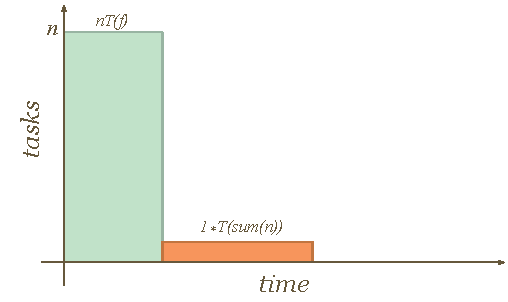
\includegraphics[scale=0.6]{figures/reduction-parallel-work.pdf}
    \end{minipage}
    $\longrightarrow$
    \begin{minipage}{.45\linewidth}
      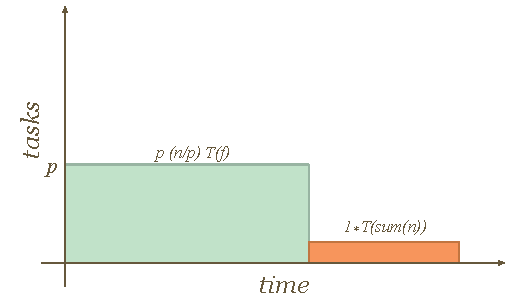
\includegraphics[scale=0.6]{figures/reduction-partitioned-work.pdf}
    \end{minipage}
%
  \item area is {\em computational work}
%
  \end{itemize}
%
\end{frame}

% --------------------------------------
% algorithmic trade-offs
\begin{frame}[fragile]
%
  \frametitle{Algorithmic improvements}
%
  \begin{itemize}
%
  \item parallelize the partial sums
    \begin{figure}
      \centering
      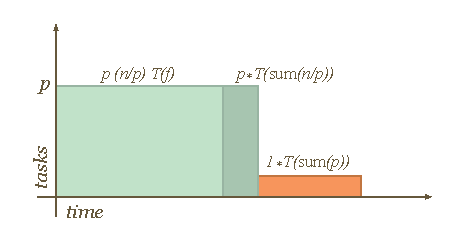
\includegraphics[scale=0.6]{figures/reduction-partial-sum.pdf}
    \end{figure}
%
  \item parallelize the final sum using a {\em reduction tree}
    \begin{figure}
      \centering
      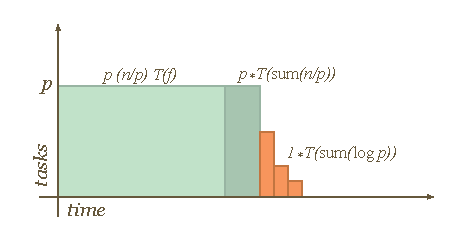
\includegraphics[scale=0.6]{figures/reduction-tree-sum.pdf}
    \end{figure}
%
  \end{itemize}
%
\end{frame}

% --------------------------------------
% load balanace
\begin{frame}[fragile]
%
  \frametitle{Load balance}
%
  \begin{itemize}
%
  \item non-optimal task distributions show up as {\em load imbalance}
    \begin{figure}
      \centering
      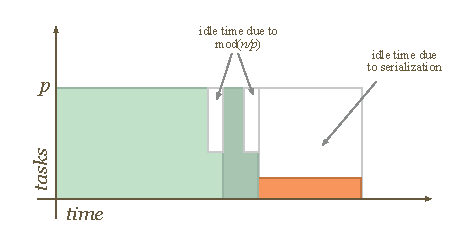
\includegraphics[scale=1.0]{figures/reduction-load-imbalance.pdf}
    \end{figure}
%
  \end{itemize}
%
\end{frame}

% --------------------------------------
% overhead
\begin{frame}[fragile]
%
  \frametitle{Parallelization overhead}
%
  \begin{itemize}
%
  \item there is always some extra work that is not present in the sequential implementation
    \begin{figure}
      \centering
      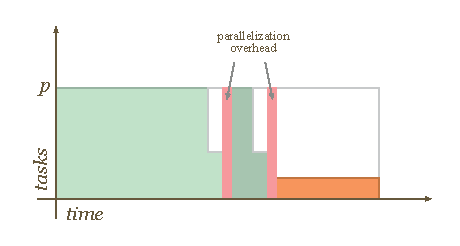
\includegraphics[scale=1.0]{figures/reduction-overhead.pdf}
    \end{figure}
%
  \end{itemize}
%
\end{frame}

% --------------------------------------
% communication and synchronization costs
\begin{frame}[fragile]
%
  \frametitle{Communication and synchronization costs}
%
  \begin{itemize}
%
  \item something something something 
    \begin{figure}
      \centering
      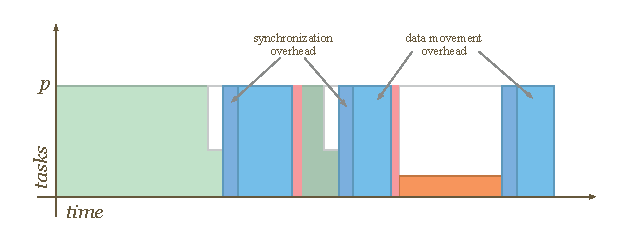
\includegraphics[scale=1.0]{figures/reduction-comsync.pdf}
    \end{figure}
%
  \end{itemize}
%
\end{frame}

% --------------------------------------
% reducing communication costs
\begin{frame}[fragile]
%
  \frametitle{Reducing communication costs}
%
  \begin{itemize}
%
  \item something something something 
    \begin{figure}
      \centering
      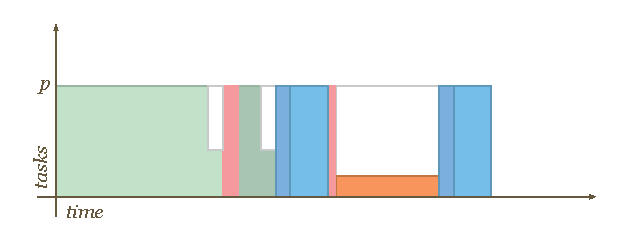
\includegraphics[scale=0.6]{figures/reduction-comsync-replication.pdf}
    \end{figure}
%
  \item something something something 
    \begin{figure}
      \centering
      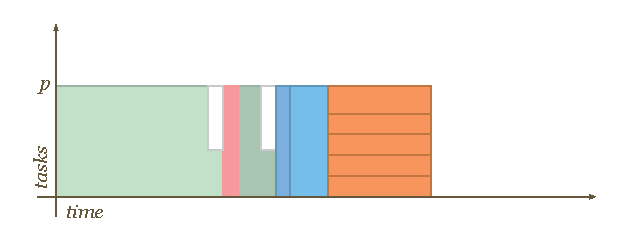
\includegraphics[scale=0.6]{figures/reduction-comsync-redundancy.pdf}
    \end{figure}
%
  \end{itemize}
%
\end{frame}

% --------------------------------------
% amdahl's law
\begin{frame}[fragile]
%
  \frametitle{Speedup}
%
  \begin{itemize}
%
  \item Amdahl's law:
    \[
    S(p) \leq \frac{1}{s+\frac{1-s}{p}} \leq \frac{1}{s}
    \]
%
  \item something something something 
    \begin{figure}
      \centering
      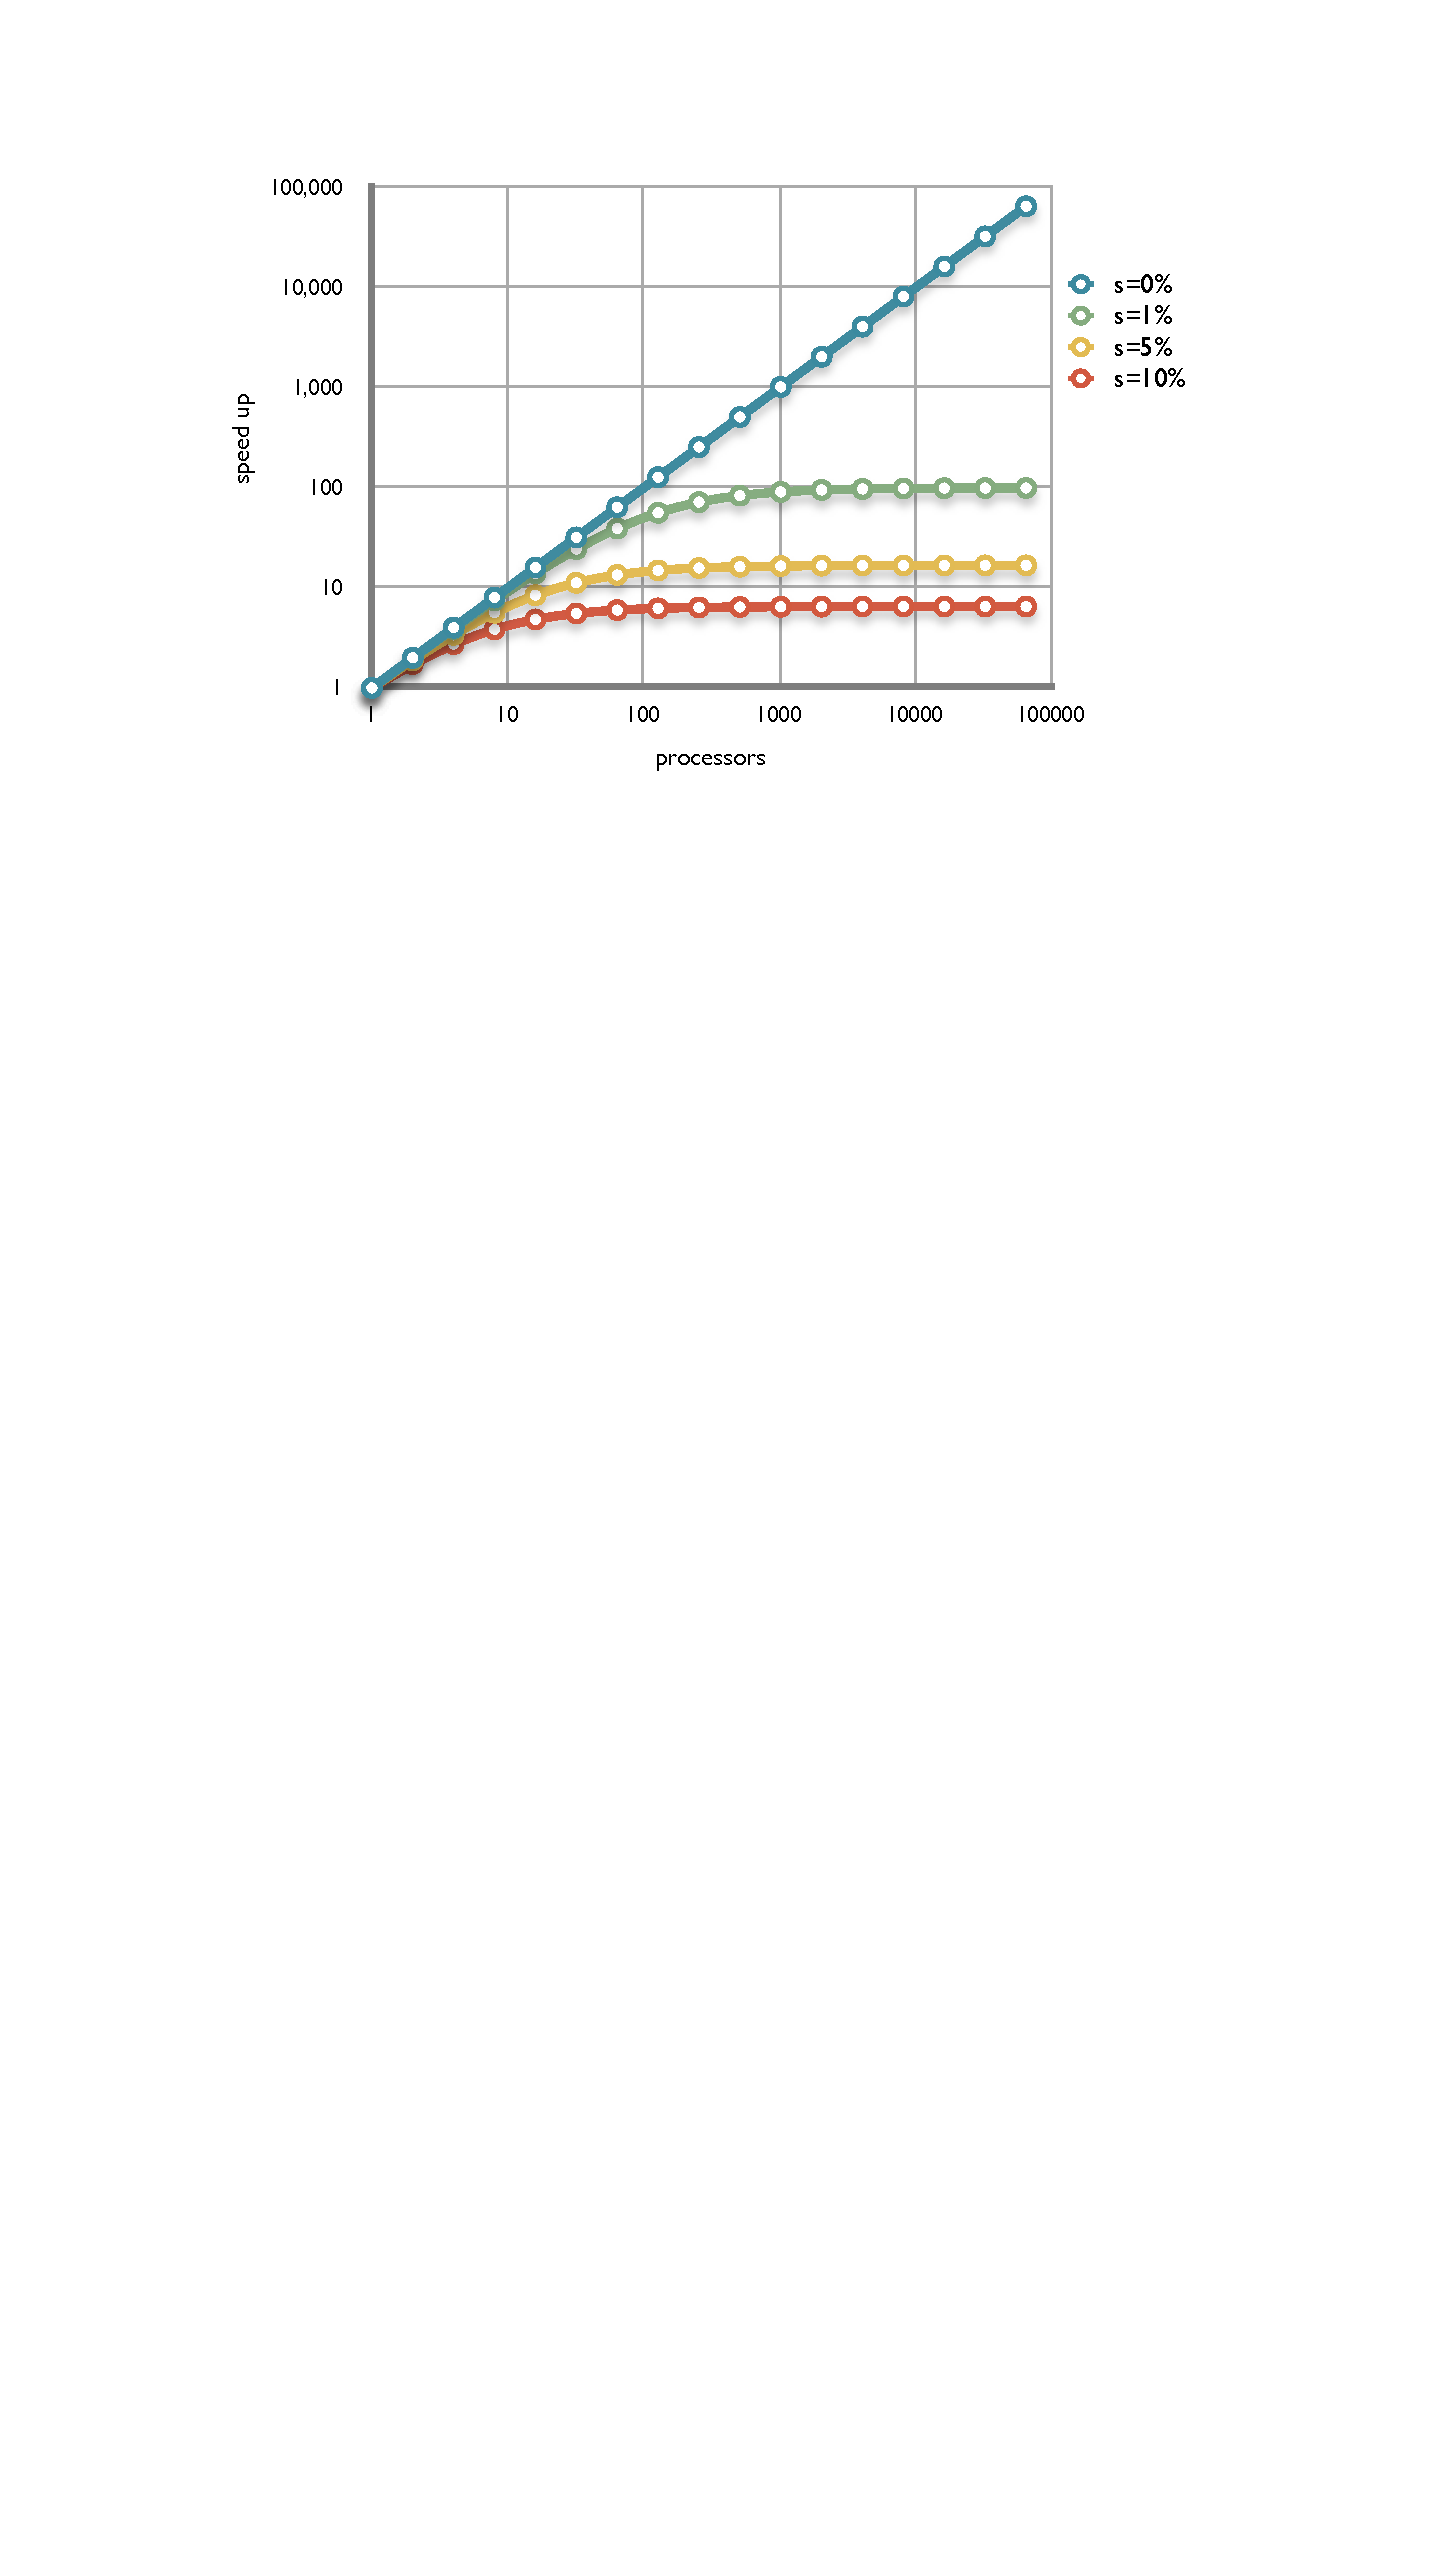
\includegraphics[scale=0.3]{figures/amdahl.pdf}
    \end{figure}
%
  \end{itemize}
%
\end{frame}

% end of file 
